\documentclass[a4paper]{article}
\usepackage{cmap}
\usepackage{mathtext}
\usepackage{amssymb}
\usepackage{amsmath}
\usepackage[russian]{babel}
\usepackage{indentfirst}
\usepackage[pdftex]{graphicx}
\usepackage{multirow}
\usepackage{siunitx}
\usepackage[left=2cm,right=2cm,top=2cm,bottom=2cm]{geometry}
\usepackage{fancyhdr}
\pagestyle{fancy}
\newcommand{\rref}[1]{(\ref{#1})}
\newcommand{\Equip}[3]{{\bf #1:} $\Delta = \pm #2$ \si{#3}

}
\newcommand{\equip}[1]{{\bf #1}

}
\newcommand{\labname}{Резонанс напряжений в последовательном контуре} 	% название пиши здесь
\newcommand{\labnum}{3.2.2.}										% номер вводи здесь
\fancyfoot{}
\fancyhead[RE, RO]{\thepage}
\fancyhead[LE, LO]{Лабораторная работа \labnum \space \labname}
\title{Лабораторная работа \labnum \space \labname} % Название работы здесь
\author{Иван Сладков}
\begin{document}
\maketitle
\thispagestyle{empty}
\section{Аннотация}
В данной работе проводится исследование колебаний напряжения в последовательном колебательном контуре под воздействием синусоидальной внешней ЭДС. Проводится определение АЧХ и ФЧХ контура; на основании этих данных определяется добротность и другие параметры контура. 

\section{Теоретические сведения}

Резонансная частота последовательного контура может быть определена из формулы
\begin{equation}\label{freq}
	f_r = \frac{1}{2 \pi \sqrt{L C}}.
\end{equation}

Добротность колебательного контура связана с его параметрами соотношениями:
\begin{equation}\label{qual}
	Q = \frac{\rho}{R_\Sigma} = \frac{\omega_0 L}{R_\Sigma} = \frac{1}{\omega_0 C R_\Sigma}.
\end{equation}

Для теоретического расчёта параметров контура используется метод комплексных амплитуд. Импеданс последовательного контура определяется по формуле:
\begin{equation}\label{импеданс}
	Z = R_\Sigma +i(\omega L - \frac{1}{\omega C}),
\end{equation}
где $ R_\Sigma $ -- суммарное активное сопротивление компонентов. $ \omega_0 $ -- резонансная частота контура, при которой импеданс -- действительный. При условии, что $ | \Delta \omega | \ll \omega_0 $, формулы резонансных значений тока и напряжения упрощаются до:
\begin{equation}\label{Ires}
	\overrightarrow{I} = \frac{E}{R_\Sigma} \frac{\exp i\varphi_I}{\sqrt{1+(\tau \Delta \omega )^2}}, 
\end{equation}
\begin{equation}\label{Ures}
	\overrightarrow{U_C} = E Q \frac{\omega_0}{\omega} \frac{\exp i \varphi_C}{\sqrt{1+\tau \Delta \omega )^2}},
\end{equation}
где 
\begin{equation*}
	\varphi_I = -\arctg (\tau \Delta \omega ), 
\end{equation*}
\begin{equation}\label{phi_c}
	\varphi_C = -\frac{\pi}{2} + \delta - \arctg (\tau \Delta \varphi ).
\end{equation}
Здесь $ \tau = 2 Q / \omega_0 $ -- время затухания колебаний.

Схожесть поведения вблизи резонанса частотных характеристик тока и напряжений на реактивных элементах последовательного контура с добротностью $ Q \gg 1 $ упрощает эксперимент, позволяя проводить измерения именно напряжений.

Резонансное напряжение определяется формулой:
\begin{equation}\label{resc}
	U_C (\omega_0) \cong Q E
\end{equation}
\begin{equation*}
	\varphi_C (\omega_0) = -\frac{\pi}{2}+\delta,
\end{equation*}
где $ \delta  $ -- малая поправка.

Заметим, что с одной стороны, $ Q \gg 1 $, так как мы пренебрегаем относительными поправками порядка $ Q^{-2} $, но с другой стороны, в контур встроен резистор для намеренного уменьшения $ Q $, чтобы упростить постройку АЧХ.
\subsection{Расчётные формулы}

Зная резонансную частоту, по формуле \eqref{freq} можно найти индуктивность катушки:
\begin{equation}\label{induct}
	L = \frac{1}{4 \pi ^2 C f^2}
\end{equation}
 Из формулы \eqref{qual} или из формулы $ \rho = \sqrt{L / C} $ можно найти реактивное сопротивление контура. Зная суммарное активное сопротивление и $ R_S = 10^{-3} \rho $, можно найти $ R_L $ -- активное сопротивление катушки. Для определения добротности контура применяется формула \eqref{Ures}.
 $ R_\Sigma $ найдём из формулы \eqref{qual}.
  
При исследовании АЧХ, будем использовать формулу
\begin{equation}\label{ACHH}
	Q = \frac{\omega_0}{\delta \omega},
\end{equation}
где $ \delta \omega $ -- ширина резонансной кривой на уровне $ U_C (\omega_0) / \sqrt{2} $.

При исследовании ФЧХ применим формулу \eqref{phi_c}: из неё, расстояние по оси $ \omega $ между точками, в которых фаза $ \varphi_C $ меняется от $ -\pi /4 $ до $ -3 \pi / 4 $, равно $ 2 / \tau $, где $ \tau  $ -- время релаксации.

\section{Оборудование и инструментальные погрешности}
На рис. \ref{set} изображена схема установки, используемой в опыте.
\begin{figure}[tb]
	\centering
	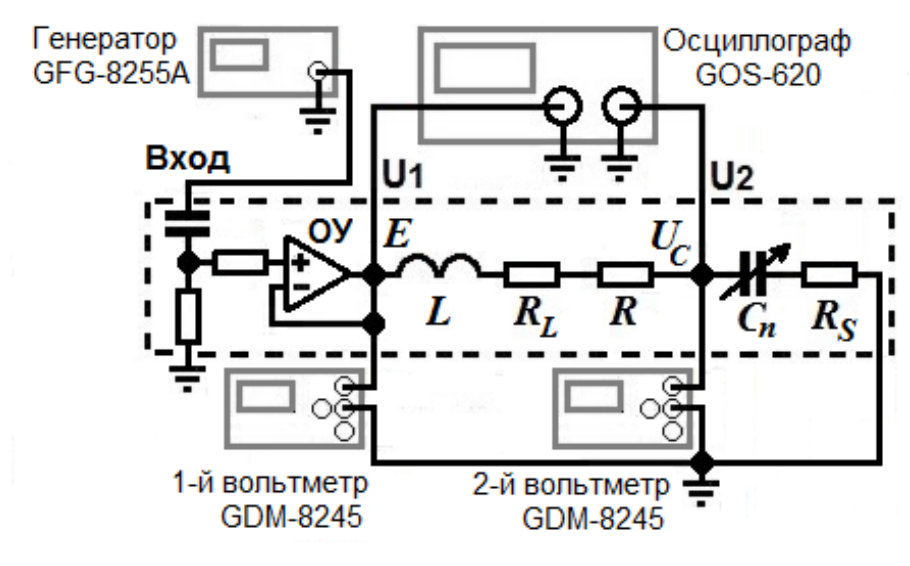
\includegraphics[width=1\linewidth]{Screenshot_1}
	\caption{Схема экспериментальной установки}
	\label{set}
\end{figure}
Синусоидальный сигнал от генератора GFG8255A поступает на вход источника напряжения, собранного на операционном усилителе ОУ. Питание операционного усилителя осуществляется встроенным блоком-выпрямителем от сети переменного тока 220 Вольт (цепь питания на схеме не показана). Источник напряжения обеспечивает с высокой точностью постоянство амплитуды сигнала на меняющейся по величине нагрузке – последовательном колебательном контуре, изображенном на рис. \ref{set} в виде эквивалентной схемы. Источник напряжения с согласующей цепочкой, колебательный контур и блок питания заключены в отдельный корпус, отмеченный на рисунке штриховой линией.

Резистор $ R $, изображённый на схеме, имеет сопротивление \SI{3.45}{\ohm}

\Equip{Генератор сигналов с частотомером}{1}{\hertz}
\equip{Последовательный колебательный контур со встроенным источником напряжения}
\Equip{Цифровые вольтметры}{10^{-4}}{\volt}
\equip{Двухлучевой осциллограф}

\section{Результаты измерений и обработка данных}
\subsection{Резонансные параметры контуров}
\label{respar}
В результате измерения резонансных частот и напряжений и последующей обработки, получены данные табл. \ref{tab:res}.
Измерения проводились для двух значений напряжения $ E $: \SI{200}{\milli \ampere} и \SI{300}{\milli \ampere}. 

\begin{table}[tb]
	\centering
	\begin{tabular}{|l|l|l|l|l|l|l|l|l|l|l|}
		\hline
		$C_n$, нФ  & $f_{0 n}$, Гц  & $U_C$, В  & $E$, В  & $L$, мкГн & $Q$  & $\rho$, Ом & $R_\Sigma$, Ом & $R_{S max}$, Ом & $R_L$, Ом & $I$, мА \\ \hline
		25         & 31950          & 5.066     & 0.2014  & 993       & 25.2 & 199        & 7.92           & 0.199           & 4.27      & 25.4    \\ \hline
		33.2       & 27754          & 4.535     & 0.2012  & 990       & 22.5 & 173        & 7.66           & 0.173           & 4.04      & 26.3    \\ \hline
		47.5       & 23245          & 3.933     & 0.2011  & 987       & 19.6 & 144        & 7.37           & 0.144           & 3.78      & 27.3    \\ \hline
		57.2       & 21180          & 3.581     & 0.201   & 987       & 17.8 & 131        & 7.37           & 0.131           & 3.79      & 27.3    \\ \hline
		67.4       & 19526          & 3.39      & 0.2009  & 986       & 16.9 & 121        & 7.17           & 0.121           & 3.60      & 28.0    \\ \hline
		82.1       & 17695          & 3.123     & 0.2007  & 985       & 15.6 & 110        & 7.04           & 0.110           & 3.48      & 28.5    \\ \hline
		99.6       & 16076          & 2.87      & 0.2005  & 984       & 14.3 & 99.4       & 6.94           & 0.0994          & 3.39      & 28.9    \\ \hline
		99.6       & 16014          & 4.252     & 0.3011  & 992       & 14.1 & 99.8       & 7.07           & 0.0998          & 3.52      & 42.6    \\ \hline
		82.1       & 17620          & 4.614     & 0.3012  & 994       & 15.3 & 110        & 7.18           & 0.110           & 3.62      & 41.9    \\ \hline
		67.4       & 19491          & 5.001     & 0.3012  & 989       & 16.6 & 121        & 7.30           & 0.121           & 3.73      & 41.3    \\ \hline
		57.2       & 21111          & 5.369     & 0.3012  & 994       & 17.8 & 132        & 7.39           & 0.132           & 3.81      & 40.7    \\ \hline
		47.5       & 23166          & 5.783     & 0.3012  & 994       & 19.2 & 145        & 7.53           & 0.145           & 3.94      & 40.0    \\ \hline
		33.2       & 27669          & 6.634     & 0.3012  & 997       & 22.0 & 173        & 7.87           & 0.173           & 4.24      & 38.3    \\ \hline
		25         & 31884          & 7.369     & 0.3011  & 997       & 24.5 & 200        & 8.16           & 0.200           & 4.51      & 36.9    \\ \hline
		\multicolumn{4}{|l|}{Среднее значение}            & 991       &      &            &                &                 & 3.84      &         \\ \hline
		\multicolumn{4}{|l|}{Стандартная ошибка среднего} & 1.1       &      &            &                &                 & 0.08      &         \\ \hline
		\multicolumn{4}{|l|}{Коэффициент Стьюдента}       & 2.4       &      &            &                &                 & 2.4       &         \\ \hline
		\multicolumn{4}{|l|}{Случайная погрешность}       & 0.28      &      &            &                &                 & 0.1       &         \\ \hline
	\end{tabular}
	\caption{Результаты измерений и обработки}
	\label{tab:res}
\end{table}

Построим векторную диаграмму на рис. \ref{diag}, отложив $ E $ по оси абсцисс с масштабом в 2 раза больше, чем по оси ординат.
Так как по закону Кирхгофа, \begin{equation}\label{kir}
	E = U_R + U_С + U_L,
\end{equation} 
на графике это равенство должно быть представлено геометрическим равенством вектора $ \mathbf{E} $ сумме остальных векторов.
\begin{figure}
	\centering
	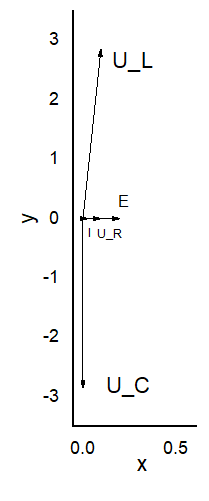
\includegraphics[height=0.4\textheight]{Screenshot_6}
	\caption{Векторная диаграмма для контура 7 при E = 0.2 В}
	\label{diag}
\end{figure}

\subsection{Исследование АЧХ}
Рассмотрим графики \ref{fig:res} и \ref{fig:resless}. Из графиков видно, что резонансная частота и добротность в контуре при $ С = \SI{67}{\nano \farad} $ ниже. 
Найдём добротность как обратное к разности частот на уровне 0.7:
\begin{equation}
	\frac{1}{Q_{C=47}} = 0.052 \pm 0.001
\end{equation}
\begin{equation}
	\frac{1}{Q_{C=67}} = 0.060 \pm 0.001
\end{equation}
\begin{equation}\label{добр1}
	Q_{C=47} = 19.2 \pm 0.1,
\end{equation}
\begin{equation}\label{добр2}
	Q_{C=67} = 16.6 \pm 0.1.
\end{equation}
Можно заметить, что добротность определённая двумя разными способами, хорошо согласуется.
\begin{figure}[tbp]
	\centering
	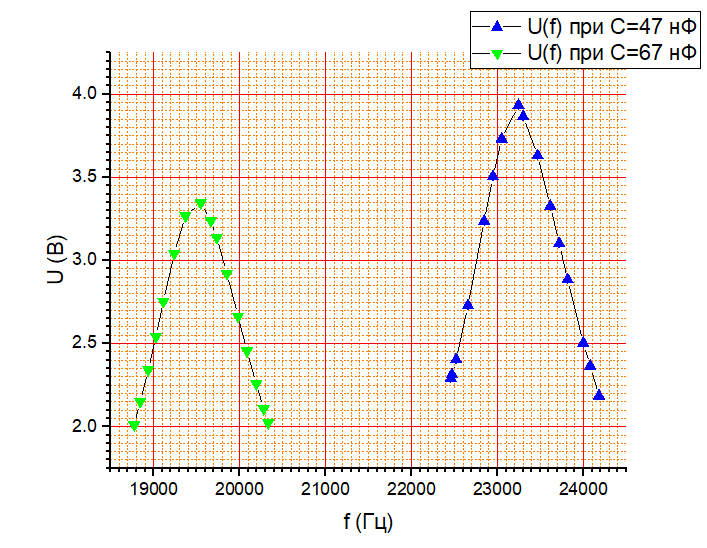
\includegraphics[width=0.8\linewidth]{Screenshot_2}
	\caption{Резонансные кривые для контуров 3 и 5}
	\label{fig:res}
\end{figure}
\begin{figure}
	\centering
	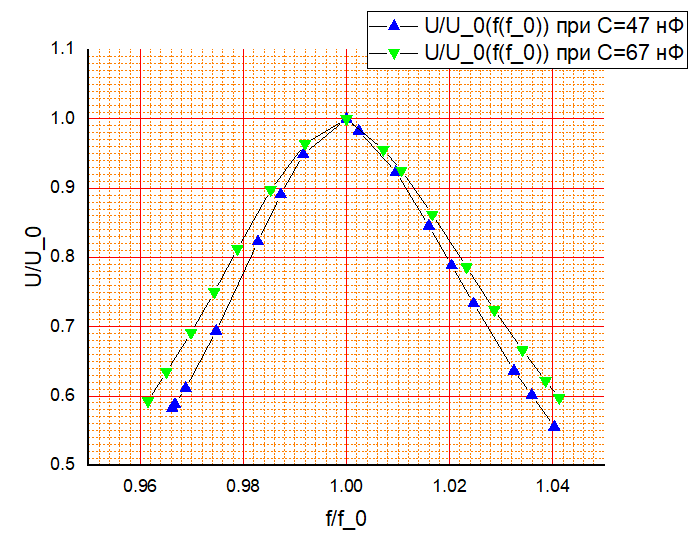
\includegraphics[width=0.8\linewidth]{Screenshot_3}
	\caption{Резонансные кривые в безразмерных координатах}
	\label{fig:resless}
\end{figure}

\subsection{Исследование ФЧХ}

По данным, полученным в ходе эксперимента, построим на рис. \ref{fchh} графики фазово-частотных характеристик для контуров 3 и 5. Графики построены в координатах $ \varphi / \pi (f/f_0) $. Определим добротность из расстояния по оси $ x $ между пересечением графиками прямых $ y = 0.25 $ и $ y = 0.75 $:
\begin{equation*}
	\frac{1}{Q_{C=47}} = 0.053 \pm 0.003
\end{equation*}
\begin{equation*}
	\frac{1}{Q_{C=67}} = 0.065 \pm 0.003
\end{equation*}
\begin{equation*}
	Q_{C=47} = 19 \pm 1
\end{equation*}
\begin{equation*}
	Q_{C=67} = 15 \pm 1
\end{equation*}
\begin{figure}[tbp]
	\centering
	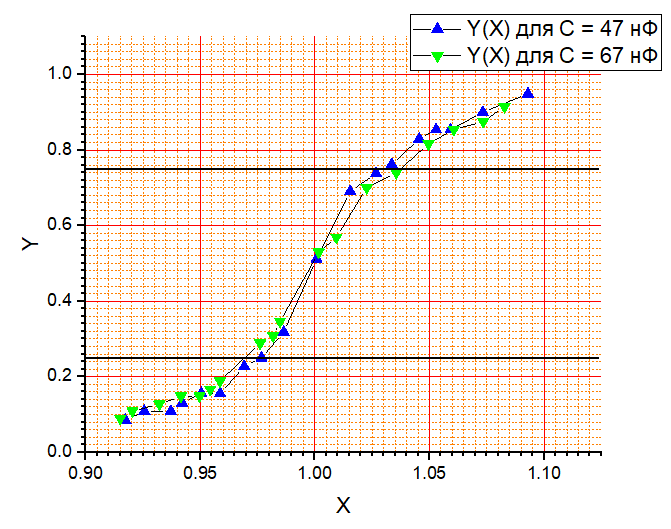
\includegraphics[width=0.8\linewidth]{Screenshot_4}
	\caption{Фазово-частотная характеристика в безразмерных координатах $ \frac{\varphi}{\pi} (f / f_0) $}
	\label{fchh}
\end{figure}

При расчёте ФЧХ становится видна ошибка в выборе контуров для исследования. Следовало выбирать контуры с наиболее различающимися характеристиками, так как иначе графики становятся менее удобными.

\subsection{Оценка погрешностей}
Так как точная регулировка генератора сигналов невозможна, и частота синусоиды меняется (убывает) со временем, погрешность генератора берём равной \SI{3}{\hertz}. По тем же причинам, погрешность вольтметра $ U_C $ берём равной \SI{1}{\milli \volt}.

Погрешность формулы \eqref{induct} определяется через:
\begin{equation}\label{sig_induct}
\sigma_L = L\sqrt{\left( \frac{\sigma_C}{C}\right)^2	+ 4\left( \frac{\sigma_f}{f}.
\right)^2}\end{equation}
Аналогично находится формула для погрешности $ Q $.

Погрешность формулы $ \rho = \sqrt{\frac{L}{C}} $ равна
\begin{equation}\label{sig_rho}
	\sigma_\rho = \rho \sqrt{\left( \frac{\sigma_L}{2L}\right)^2+\left( \frac{\sigma_C}{2C}\right)^2}
\end{equation}

Все погрешности, рассчитанные в пункте \ref{respar}, занесены в табл. \ref{погр}.

При вычислении погрешностей АЧХ и ФЧХ, случайные погрешности косвенных измерений существенно меньше, чем погрешность метода (так как необходимо определить добротность по графику). В частности, для АЧХ $ \sigma_Q = 0.01 $ Поэтому взята погрешность равная половине цены деления обоих графиков.

\begin{table}[h]
	\centering
	\begin{tabular}{|l|l|l|l|l|l|l|l|l|l|}
		\hline
		$\sigma_{C_n}$, нФ & $\sigma_{f_{0 n}}$, Гц & $\sigma_{U_C}$, В & $\sigma_E$, В & $\sigma_L$, мкГн & $\sigma_Q$ & $\sigma_\rho$, Ом & $\sigma_{R_\Sigma}$, Ом & $\sigma_{R_L}$, Ом & $\sigma_I$, мА \\ \hline
		0.1                & 3                      & 0.001             & 1E-4          & 4.0              & 0.013      & 0.56              & 0.02                    & 0.02               & 0.07           \\ \hline
		0.1                & 3                      & 0.001             & 1E-4          & 3.0              & 0.012      & 0.37              & 0.02                    & 0.02               & 0.06           \\ \hline
		0.1                & 3                      & 0.001             & 1E-4          & 2.1              & 0.011      & 0.22              & 0.01                    & 0.02               & 0.05           \\ \hline
		0.1                & 3                      & 0.001             & 1E-4          & 1.7              & 0.010      & 0.16              & 0.01                    & 0.01               & 0.04           \\ \hline
		0.1                & 3                      & 0.001             & 1E-4          & 1.5              & 0.0098     & 0.13              & 0.009                   & 0.01               & 0.04           \\ \hline
		0.1                & 3                      & 0.001             & 1E-4          & 1.2              & 0.0092     & 0.096             & 0.007                   & 0.01               & 0.03           \\ \hline
		0.1                & 3                      & 0.001             & 1E-4          & 1.1              & 0.0087     & 0.073             & 0.007                   & 0.01               & 0.03           \\ \hline
		0.1                & 3                      & 0.001             & 1E-4          & 1.1              & 0.0057     & 0.073             & 0.006                   & 0.01               & 0.04           \\ \hline
		0.1                & 3                      & 0.001             & 1E-4          & 1.3              & 0.0061     & 0.097             & 0.007                   & 0.01               & 0.04           \\ \hline
		0.1                & 3                      & 0.001             & 1E-4          & 1.5              & 0.0064     & 0.13              & 0.008                   & 0.01               & 0.05           \\ \hline
		0.1                & 3                      & 0.001             & 1E-4          & 1.8              & 0.0068     & 0.16              & 0.010                   & 0.01               & 0.05           \\ \hline
		0.1                & 3                      & 0.001             & 1E-4          & 2.1              & 0.0072     & 0.22              & 0.01                    & 0.02               & 0.06           \\ \hline
		0.1                & 3                      & 0.001             & 1E-4          & 3.0              & 0.0080     & 0.37              & 0.02                    & 0.02               & 0.08           \\ \hline
		0.1                & 3                      & 0.001             & 1E-4          & 4.0              & 0.0088     & 0.57              & 0.02                    & 0.03               & 0.1            \\ \hline
	\end{tabular}
	\caption{Погрешности первого эксперимента}
	\label{погр}
\end{table}

\section{Вывод}
Проведено исследование колебаний напряжения в последовательном контуре. Несколькими методами была определена добротность контуров. Результаты неплохо согласуются.

Построен график $ R_L (f_0) $ на рис. \ref{ind}. Видно, что сопротивление меняется практически линейно. Можно предположить, что изменения связаны с потерями на перемагничивание сердечника катушки. 

 
\begin{figure}
	\centering
	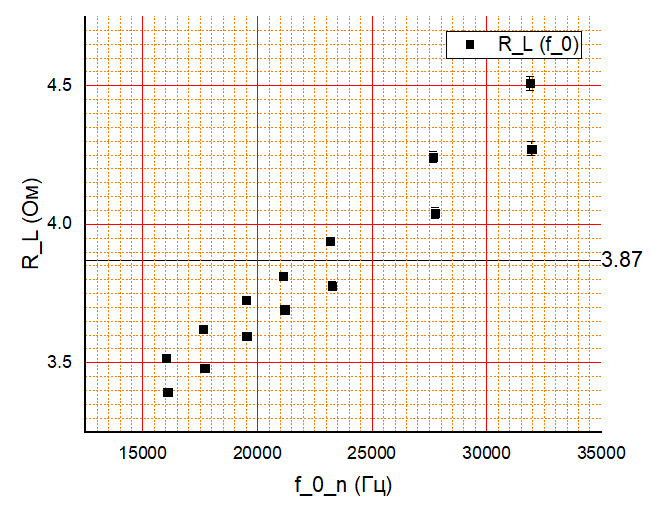
\includegraphics[width=0.8\linewidth]{Screenshot_5}
	\caption{График изменения активного сопротивления индуктивности}
	\label{ind}
\end{figure}


\begin{thebibliography}{9}
\bibitem{Siv} Сивухин Д. В. \emph{Общий курс физики. Том 3 Электричество и магнетизм}, 2004
\bibitem{kirich} Кириченко Н.А. \emph{Электричество и магнетизм.}, 2011
\end{thebibliography}
\end{document}

